\documentclass{beamer}
\usepackage[T1]{fontenc}
\usepackage[utf8]{inputenc}
\usepackage{lmodern} 
\usepackage[portuguese]{babel}
\usepackage{graphicx}			%para imagens
\usepackage{epstopdf} 			%resolve problemas eps-pdf
\usepackage{fancyhdr}			% para o cabeçalho bonito
\usepackage{caption}				%para legendas
\usepackage{placeins} 			%controlar o lugar dos floats
\usepackage{hyperref}
\usepackage{listings}
\usepackage{color}
\usepackage{xcolor}

\definecolor{dkgreen}{rgb}{0,0.6,0}
\definecolor{gray}{rgb}{0.5,0.5,0.5}
\definecolor{mauve}{rgb}{0.58,0,0.82}

\lstset{frame=tb,
  language=Java,
  aboveskip=3mm,
  belowskip=3mm,
  showstringspaces=false,
  columns=flexible,
  basicstyle={\tiny\ttfamily},
  numbers=none,
  numberstyle=\tiny\color{gray},
  keywordstyle=\color{blue},
  commentstyle=\color{dkgreen},
  stringstyle=\color{mauve},
  breaklines=true,
  breakatwhitespace=true
  tabsize=3
}
\lstset{language=Java}

\defbeamertemplate*{title page}{customized}[1][]
{
  \usebeamerfont{title}\inserttitle\par
  \usebeamerfont{subtitle}\usebeamercolor[fg]{subtitle}\insertsubtitle\par
  \bigskip
 %% \usebeamerfont{author}\insertauthor\par
  \usebeamerfont{institute}\insertinstitute\par
  \usebeamerfont{date}\insertdate\par
  \usebeamercolor[fg]{titlegraphic}\inserttitlegraphic
}

%DEFINE TEMA BEAMER A SER UTILIZADO
\usetheme{Warsaw}
\setbeamertemplate{navigation symbols}{}%remove navigation symbols
%DEFINIÇÃO DE TÍTULO, AUTORES .....
\title[Introdução a Computação Sônica]{ ICS - Trabalho II \\ Síntese Aditiva}
%\title[pequeno título que vai no bottom da página]{título grande}%
\author{Juarez Aires Sampaio Filho 11/0032829}
\institute{Universidade de Brasília}
\date{\today}

\begin{document}


\begin{frame}
        \titlepage
\end{frame}

\AtBeginSection[]
{
%%página com layout da sessão ao início de cada sessão
 \begin{frame}<beamer>
   \tableofcontents[currentsection,currentsubsection]
 \end{frame}
}
\section{Requisitos}
\begin{frame}{Requisitos}
	\frametitle{Requisitos}
    \begin{itemize}
	\item Desenvolver uma interface gráfica em Java que implemente três instrumentos aditivos(ver figura a seguir) 
	e seja capaz de tocar melodias e notas com ele. A interface deve possuir operações de:
	\begin{itemize}
	 \item Música: tocar uma melodia ou ruídos interessantes
	 \item Nota
	 \end{itemize}
    \end{itemize}
\end{frame}

\begin{frame}
 \frametitle{Dispositivo RAN}
 \begin{figure}
  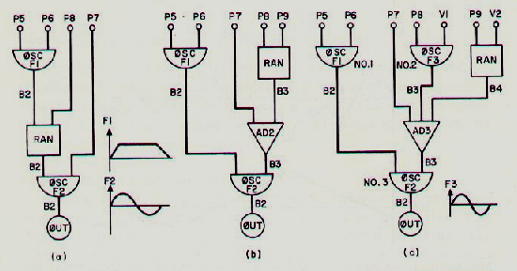
\includegraphics[scale=0.6]{./images/meusInstrumentos.png}
  \caption{Instrumentos a serem implementados}
   \end{figure}
\end{frame}

\section{Classes Desenvolvidas}
\subsection{Dispositivo RAN}
\begin{frame}[fragile]
	\frametitle{RAN}
	\begin{itemize}
		\item Vemos pelas especificações que \textbf{RAN precisa aceitar} como entrada
		tanto uma \textbf{constante} como um \textbf{dispositivo}.
		\item Dentre as classes disponíveis na API SomA, escolhemos fazer isso utilizando como base a classe \textbf{Oscilador}
		\item Essa é a escolha natural para ter como classe base
		\item Gostaríamos de poder setar a tabela SIN da classe oscilador
		para aquela tabela gerada com números aleatório. Como isso não é possível,
		\textbf{foi necessário uma gambiarra}.
		\item \textbf{A frequência do sin é setada para 0 e sua fase para 90}. Desta forma temos um sinal constante em +1
		\item a entrada da amplitude é um dispositivo multiplicador
		\item as entradas desse multiplicador são duas envoltórias: Uma é gerada
		aleatoriamente em -1 e +1 e a outra é uma envoltória de amplitude gerada pelo usuário
	\end{itemize}
\end{frame}

\begin{frame}
 \frametitle{Dispositivo RAN}
 \begin{figure}
  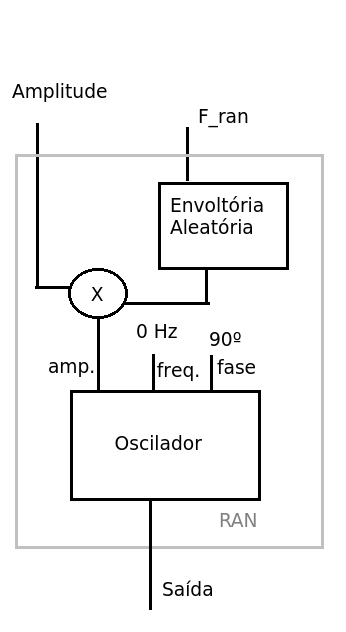
\includegraphics[scale=0.3]{./images/RAN.png}
  \caption{Dispositivo RAN: esquemático da construção}
   \end{figure}
\end{frame}

\begin{frame}[fragile]
	\frametitle{RAN}
Classe desenvolvida para gerar a envoltória aleatória.	
	\begin{itemize}
		\item extends \textbf{Oscilador}
		\item entradas controláveis: 
		\begin{itemize}
			\item f\_ruido: define o número de amostras aleatórias geradas no intervalo
			\item a: define a amplitude da envoltória gerada. Isto é, os números aleatórios vão de -A até +A. Pode ser uma constante ou um objeto Envoltoria.
		\end{itemize}
		\item fórmula utilizada para gerar números entre -A e +A :
		\begin{tiny}	\begin{lstlisting}
				float random = 2f*A*((float)Math.random()) - A;		    				
		\end{lstlisting} \end{tiny}	
		
		\item possui método de visualização gerado com o pacote \textbf{jmathtool}			
	\end{itemize}
\end{frame}



\begin{frame}
 \frametitle{Dispositivo RAN - Detalhes}
 \begin{itemize}
 	\item A frequência f\_ruido nos dá o intervalo com que os pontos aleatório são gerados
 	em uma tabela onde a última posição é 720.
 	\item Isto é, os pontos são gerados em intervalos de $\frac{720}{f\_ruido}$
 	\item Ou seja, f\_ruido define o número de amostras aleatórias presentes na duração
 	de \textbf{toda} a envoltória.
 	\item \textbf{A sensação do ruído, no entanto, é sentida pela quantidade de pontos aleatórios em 1 segundo}.
 	\item Para mantermos a mesma sensação, é\textbf{ necessário alterar a frequência do ruído} quando a duração da nota for alterada, \textbf{de modo que dentro de 1 segundo tenhamos o mesmo
 	número de pontos aleatórios} que tínhamos antes.
 	\item Usamos então de uma variável para f\_ran\_atual e outra para f\_ran\_base
 \end{itemize}
\end{frame}

\begin{frame}
 \frametitle{Dispositivo RAN}
 \begin{figure}
  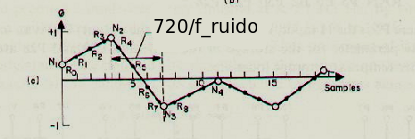
\includegraphics[scale=1.0]{./images/f_ruido.png}
  \caption{f\_ruido define o intervalo com que os pontos aleatório são gerados}
   \end{figure}
\end{frame}

\begin{frame}
 \frametitle{Dispositivo RAN}
 \begin{figure}
  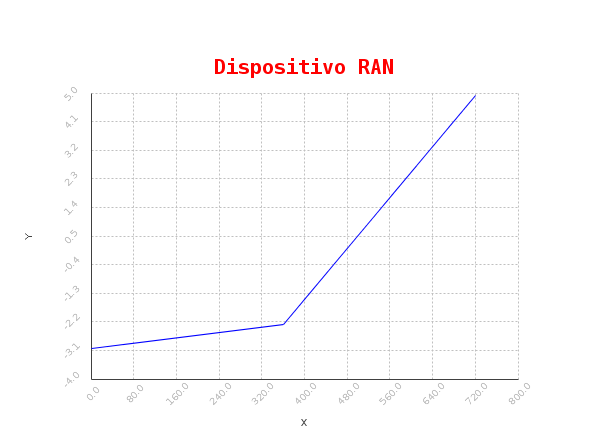
\includegraphics[scale=0.4]{./images/RAN_F_2.png}
  \caption{Dispositivo RAN, f\_ran = 2, A = 10}
   \end{figure}
\end{frame}

   \begin{frame}
 \begin{figure}
  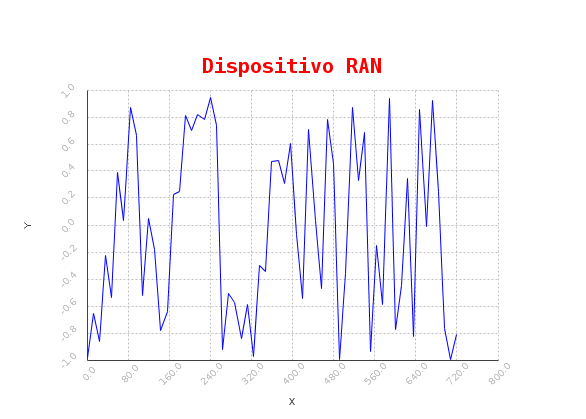
\includegraphics[scale=0.4]{./images/RAN_F_60.png}
  \caption{Dispositivo RAN, f\_ran = 60, A = 1}
 \end{figure} 
\end{frame}

 \begin{frame}[fragile]
 \frametitle{RAN - detalhes}
 \begin{figure}
 	\begin{lstlisting}
	private void setRAN(){
		setFrequencia(0);
		setFase(90);
		envFinal = new Multiplicador(randomEnv, ganhoEnv);
		setDispositivoAmplitude(envFinal);
	}
    			\end{lstlisting}
    			
    			\caption{detalhes do método de configuração}
	\end{figure}
\end{frame}

 \begin{frame}[fragile]
 \frametitle{RAN - detalhes}
 \begin{figure}
 	\centering
 	\begin{lstlisting}
	public void setDuracao(float d){
		ganhoEnv.setDuracao(d);
		this.duracao =  d;
		f_ruido = d*f_ruido_base;
		generateRandomEnv();
		randomEnv.setDuracao(d);
	}
    			\end{lstlisting}
	\caption{detalhes do método para configurar duração}	
	\end{figure}
\end{frame}
\subsection{Instrumento 1}
\begin{frame}
 \frametitle{Instrumento 1}
 \begin{itemize}
 \item Extends \textbf{UnidadeH}
 \item Como a unidade H é o menor instrumento possível, nossos instrumentos são todos
 descendentes dela.
 \item Criamos uma unidadeH com \textbf{super()} e pegamos o seu oscilador.
 \item setamos então a entrada de ganho o oscilador para um dispositivo \textbf{RAN}
 \item redefinimos então os métodos \textbf{setGanho} e \textbf{setDuracao} para atuarem no objeto \textbf{RAN}
 \end{itemize}
\end{frame}

 \begin{frame}[fragile]
 \frametitle{Instrumento 1 - construção}
 \begin{figure}
 	\centering
 	\begin{lstlisting}
	public Instrumento1(){
		super();
		initialize(); //inicializa as variaveis

		setH(1.0f);
		setGanho(1f);
		setLambda(0.5f);
		
		ran.setGanho(env);
		ran.setGanho(10);
		ran.setF_ruido(60);
		osci.setDispositivoAmplitude(ran);
		osci.setFrequencia(440);
		osci.setDuracao(5f);
	}
    			\end{lstlisting}
	\caption*{}	
	\end{figure}
\end{frame}

\begin{frame}
 \begin{figure}
  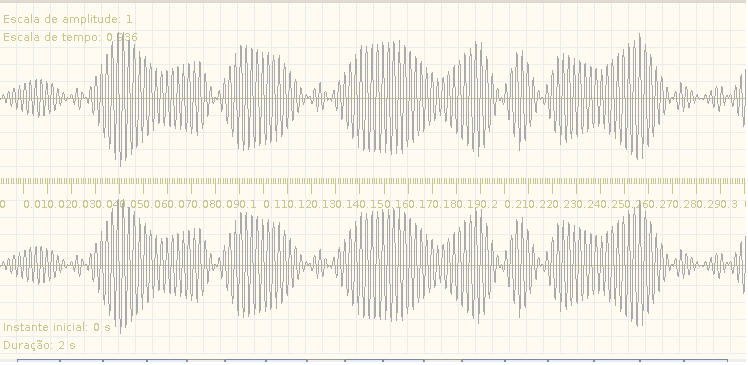
\includegraphics[scale=0.4]{./images/ins1.png}
  \caption{Saída do Instrumento 1}
 \end{figure} 
\end{frame}
\subsection{Instrumento 2}
\begin{frame}
 \frametitle{Instrumento 2}
 \begin{itemize}
 \item Extends \textbf{UnidadeH}
 \item \textbf{Basta conectar os blocos}.
 \item A figura a seguir ilustra a conexão entre os blocos.
 \end{itemize}
\end{frame}

\begin{frame}
 \begin{figure}
  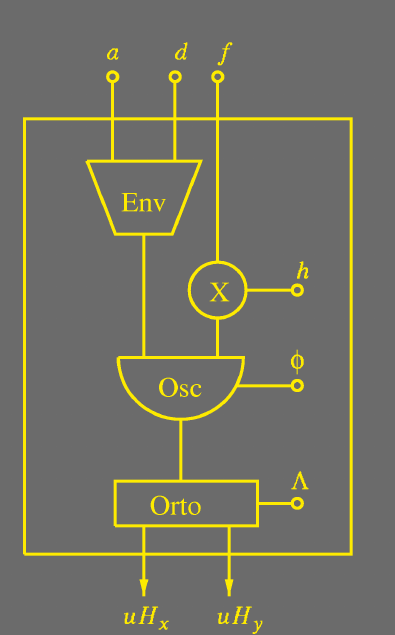
\includegraphics[scale=0.3]{./images/unidadeH.png}
  \caption{Unidade H padrão: no trabalho desenvolvido, não utilizamos a env padrão
  da unidade H}
 \end{figure} 
\end{frame}

\begin{frame}
 \begin{figure}
  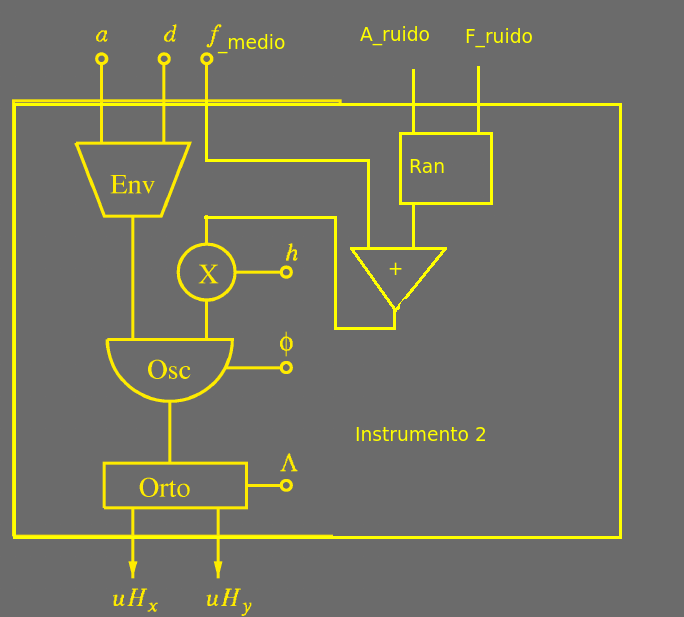
\includegraphics[scale=0.4]{./images/instrumento2.png}
  \caption{Esquemático do instrumento 2 tendo como base a unidade H}
 \end{figure} 
\end{frame}
 \begin{frame}[fragile]
 \frametitle{Instrumento 2 - construção}
 	\begin{lstlisting}
public Instrumento2(){
		super();
		setLambda(0.5f);
		ran = new RAN(20f, 10);
		f_medio = 440;
		f_medio_env = constantEnvoltoria(f_medio);
		sum = new Somador(f_medio_env, ran);

		//define envoltoria padrao
		Curva curva = new Curva(720);
		curva.addPonto(0f, 0f);
		curva.addPonto(60f, 1000f);
		curva.addPonto(450f, 1000f);
		curva.addPonto(720f, 0f);
		ganhoEnv = new Envoltoria();
		ganhoEnv.setCURVA(curva);

		
		osci = getOscilador();
		osci.setDispositivoAmplitude(ganhoEnv);
		osci.setDispositivoFrequencia(sum);
	}
	    			\end{lstlisting}
\end{frame}

\begin{frame}
 \begin{figure}
  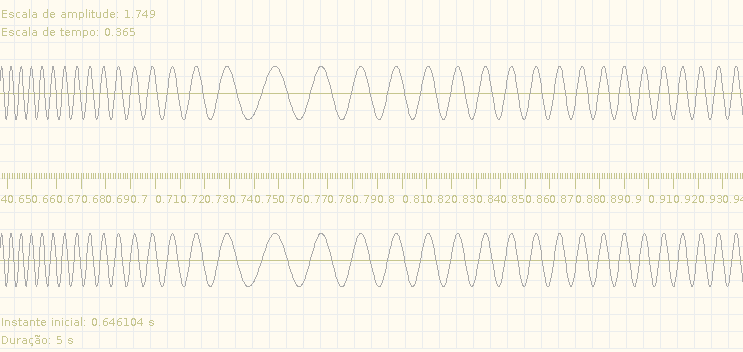
\includegraphics[scale=0.4]{./images/ins2.png}
  \caption{Saída do Instrumento 2}
 \end{figure} 
\end{frame}

\subsection{Instrumento 3}
\begin{frame}
 \frametitle{Instrumento 3}
  \begin{itemize}
 \item Extends \textbf{UnidadeH}
 \item Como no item anterior, \textbf{basta conectar os blocos necessários}.
 \item Pode ser visto como uma extensão do Instrumento 2. As classes são muito semelhantes.
 \item Apenas acrescentamos um somador e um oscilador ao instrumento 2.
 \end{itemize}
\end{frame}

\begin{frame}
 \begin{figure}
  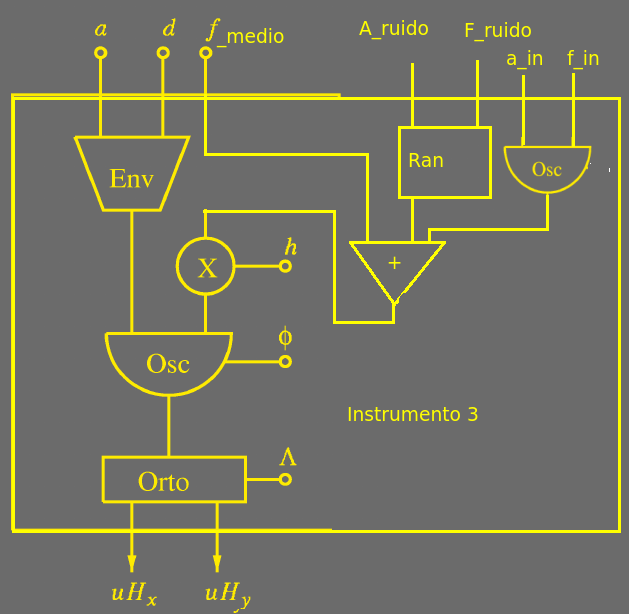
\includegraphics[scale=0.4]{./images/instrumento3.png}
  \caption{Esquemático do instrumento 3 tendo como base a unidade H}
 \end{figure} 
\end{frame}


 \begin{frame}[fragile]
 \frametitle{Instrumento 3 - construção}
 \begin{figure}
 	\centering
 	\begin{lstlisting}
public Instrumento3(){
		//propriedades da unidadeH
		super();
		setLambda(0.5f);
		//RAN
		ran = new RAN(100f, 10);//RAN(float amplitude, float new_f_ran)		
		//Frequencia media
		f_medio = 440;
		f_medio_env = constantEnvoltoria(f_medio);
		//F medio + RAN
		sum1 = new Somador(f_medio_env, ran);
		osciF = new Oscilador(1, 1, 0); //Oscilador(float a, float f, float p) 
		sum2 = new Somador(sum1, osciF);
		//define envoltoria padrao
		Curva curva = new Curva(720);
		curva.addPonto(0f, 0f);
		curva.addPonto(60f, 1000f);
		curva.addPonto(450f, 1000f);
		curva.addPonto(720f, 0f);
		ganhoEnv = new Envoltoria();
		ganhoEnv.setCURVA(curva);
		osci_out = getOscilador();
		osci_out.setDispositivoAmplitude(ganhoEnv);
		osci_out.setDispositivoFrequencia(sum2);
	}    			\end{lstlisting}
	\caption{}	
	\end{figure}
\end{frame}


\begin{frame}
 \begin{figure}
  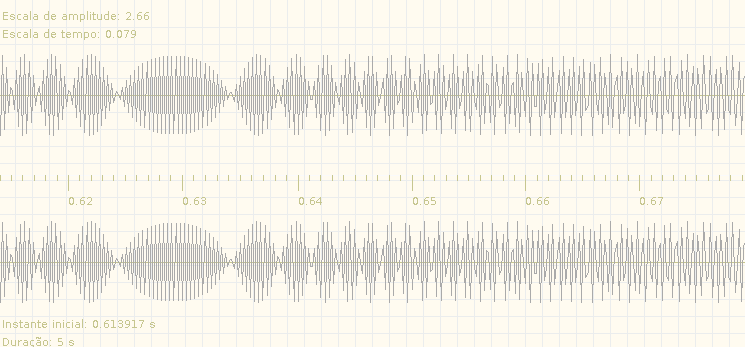
\includegraphics[scale=0.4]{./images/ins3.png}
  \caption{Saída do Instrumento 3}
 \end{figure} 
\end{frame}

\subsection{Instrumento}
\begin{frame}
 \frametitle{Instrumento}
 \begin{itemize}
 \item Uma interface que os dispositivos anteriores devem interpretar
 \item Possui métodos básicos que todos os instrumentos devem possuir
 \item Facilita a manipulação de diferentes instrumentos dentro da interface gráfica
 \end{itemize}
\end{frame}


\section{Interface Gráfica em JAVA}

\begin{frame}
	\begin{block}{Interface Gráfica}
	Desenvolveu-se uma interface simples capaz de setar todos
	os parâmetros dos instrumentos, selecionar diferentes instrumentos e
	setar parâmetros pre-definidos para gerar sons interessantes	
	\end{block}
 \begin{figure}
  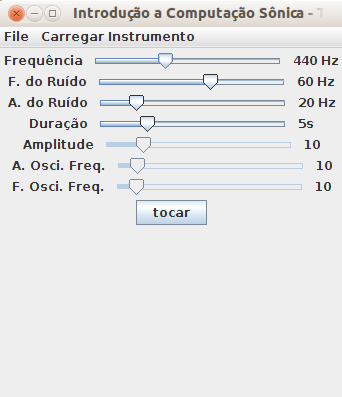
\includegraphics[scale=0.4]{./images/interface.png}
  \caption{Interface gráfica desenvolvida}
 \end{figure} 
	
 
\end{frame}


\section{Documentação e Referências}
\begin{frame}
  \frametitle{Documentação e Referências}
  \begin{itemize}
  \item \href{/home/juarez408/Documents/GitHub/GitCode/UnB2014/ICS/Trabalho2/doc/index.html}{Documentação produzida com javadoc}
  \item \href{http://www.cic.unb.br/docentes/lcmm/sintese/javadoc/}{Documentação da API sintese}
  \item \href{https://code.google.com/p/jmathplot/}{API jmathplot}
  \end{itemize}
\end{frame}



\end{document}
